% !Mode:: "TeX:UTF-8"
% !Mode:: "TeX:UTF-8"
% !TEX root = tjumain.tex


\baselineskip=20pt

\chapter{绪论}
\section{第一节}
\subsection{第三级标题}
《他改变了中国:江泽民传》(如图~\ref{book}~所示)这本传记介绍了江泽民同志的人生历程,尤其是阐述和评价了江泽民同志担任中国主要领导人的10多年中创立的历史功绩。在着重于国事活动的同时,也广泛涉及家庭生活、业余爱好、人品风格等方方面面,多角度、多侧面地展现了传主的风采。

	\begin{figure}[htbp!]
		\centering
		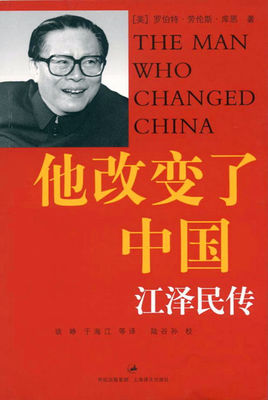
\includegraphics[width=0.5\textwidth]{figures/The_Man_Who_Changed_China.png}
		\caption{红宝书封面}\label{book}
		\vspace{-1em}
	\end{figure}	



\chapter{怒斥记者}
我觉得你们啊,你们……我感觉你们新闻界还要学习一个,你们非常熟悉西方的这一套value。你们毕竟还图样,明白这意思吧。我告诉你们我是身经百战了,见得多啦!啊,西方的哪一个国家我没去过?媒体他们——你……你们要知道,美国的华莱士,那比你们不知道高到哪里去了。啊,我跟他谈笑风生!所以说媒体啊,要……还是要提高自己的姿势水平!懂我的意思——识得唔识得啊?唉,我也给你们着急啊,真的。你们真的……我以为……遍地……你们有一个好,全世界跑到什么地方,你们比其他的西方记者啊,跑得还快。但是呢,问来问去的问题啊,都图森破,啊,上台拿衣服!懂了没有啊?识得唔识得啊?

我很抱歉,我今天是作为一个长者给你们讲的。我不是新闻工作者,但是我见得太多了,我……我有这个必要告诉你们一点,人生的经验。我刚才呢……我刚才我很想啊,就是我每一次碰到你们我就讲中国有一句话叫“闷声大发财”,我就什么话也不说。这是坠吼滴!但是我想,我见到你们这样热情啊,一句话不说也不好。所以你刚才你一定要——在宣传上将来如果你们报道上有偏差,你们要负责的。我没有说要钦定,没有任何这个意思。但是你问……你一定要非得要问我……对董先生姿瓷不姿瓷。我们不姿瓷他?他现在是当特首,我们怎么能不姿瓷特首?对不对?

\begin{lstlisting}[language=Java,caption={一个典型的测试函数},label=testFunc:add]
public void testDecimal() {
	int a=1,b=2;
	BigDecimal a = new BigDecimal(a);
	BigDecimal b = new BigDecimal(b);
	BigDecimal sum = a.add(b);
	assertEquals(sum , new BigDecimal(a+b));
	}
\end{lstlisting}

\begin{table}[htbp]
	\caption{长者用语对照表}\label{table}
	\vspace{0.5em}\centering\wuhao
	\begin{tabular}{ccccc}
		\toprule[1.5pt]
		原文 & 翻译 \\
		\midrule[1pt]
		吼哇 & 好啊 \\
		姿瓷 & 支持 \\
		姿势水平 & 知识水平 \\
		图样 & too young \\
		图森破 & too simple \\
		上台拿衣服 & sometimes naive \\
		识得唔识得啊 & 知道不知道啊 \\
		捉鸡 & 着急 \\
		这是坠吼滴 & 这是最好的 \\
		安格瑞 & angry \\
		一颗赛艇 & excited \\
		\bottomrule[1.5pt]
	\end{tabular}
	\vspace{\baselineskip}
\end{table}



\chapter{视察二院}
\section{我的经历}
我的这个经历就是到了上海,到了89年的年初的时候,我在想我估计是快要离休了,我想我应该去当教授。于是我就给朱物华校长、张钟俊院长,给他们写了一个报告。他们说欢迎你来,不过,这个Apply for Professor,你要去做一个报告。我就做了一个能源与发展趋势的主要的节能措施\citeup{江泽民1989能源发展趋势及主要节能措施},这个报告经过好几百个教授一致通过。那么上海交大教授当了以后我就做第二个报告,就是微电子工业的发展\citeup{江泽民1989论世界电子信息产业发展的新特点与我国的发展战略问题}。这两个报告做了以后不久,过后,1989年的5月31号北京就把我调到北京去了。现在这个报告做了快20年了,所以呢我就去年呢在我们交大的学报,我发表了两篇文章\citeup{江泽民2008对中国能源问题的思考,江泽民2008新时期我国信息技术产业的发展},就是呼应这个89年的报告的。特别是昨天晚上,他又把我这个第二篇报告,还有我这十几年包括在电子工业部、上海市所做的有关于信息产业化的文章,总共我听他们讲是27篇……我也没有什么别的东西送给你们,我们拿来以后我叫钱秘书啊,就把这两个学报,两个学报的英文本——因为他们这里洋文好的人多得很哪——英文本,还有前面出过两本书,再加上昨天晚上出的这本书,送给郭伟华同志,给你送过来,那么给你们作为一个纪念。

\section{不可预料}
人呐就都不知道,自己就不可以预料。一个人的命运啊,当然要靠自我奋斗,但是也要考虑到历史的行程。我绝对不知道,我作为一个上海市委书记怎么把我选到北京去了,所以邓小平同志跟我讲话,说“中央都决定啦,你来当总书记”,我说另请高明吧。我实在我也不是谦虚,我一个上海市委书记怎么到北京来了呢?但是呢,小平同志讲“大家已经研究决定了”,所以后来我就念了两首诗,叫“苟利国家生死以,岂因祸福避趋之”,那么所以我就到了北京。

\section{三件小事}
到了北京我干了这十几年也没有什么别的,大概三件事:

\begin{itemize}
	\item 一个,确立了社会主义市场经济;
	\item 第二个,把邓小平的理论列入了党章;
	\item 第三个,就是我们知道的“三个代表”。
\end{itemize}

如果说还有一点什么成绩就是军队一律不得经商!这个对军队的命运有很大的关系。因为我后来又干了一年零八个月,等于我在部队干了15年军委主席。还有九八年的抗洪也是很大的。但这些都是次要的,我主要的我就是三件事情,很惭愧,就做了一点微小的工作,谢谢大家。



\chapter{谈笑风生}
新闻、媒体也是企业,它们不是非赢利组织,而是以赢利为目的的商业企业。新闻是这些企业制造的产品,它们想用新闻这个产品去赚钱,它们就有充分的动机弄虚做假、以次充好、串谋合谋、唯利是图。凭什么新闻这个产品的质量就可以不受监管、不受控制呢?在新闻质量和新闻消费者之间不是一样存在一个信息非对称问题吗?看来,美国这个先进国家还没有想出监管新闻这种产品的好办法来,就象你们在30年代以前对商业自由那样,既然如此,我们有什么必要匆匆忙忙去抄袭你们呢?还是等你创造出更好的经验后,我们再去学习吧。

至于个人自由,任何人的绝对自由都是对别人的限制。美国南部有个工厂,白种工人在车上画着南方联邦的旗帜,非裔工人向厂方提出抗议,厂方同意不让这些车进厂门,白种工人又抗议他们的言论自由受到侵害。倒底谁应该有言论自由的权力呢?双方都有就会产生冲突,一方有,另一方就会受到限制。有一个人烧了美国国旗,地方法院要起诉他,最高法院认为这个人无罪,因为他有言论自由的权力。而美国国会的一些议员不干了,他们要立法使这个人有罪。倒底谁说的对呢?所谓言论自由,本质上是一个博奕论难题,没有正确的解,所以要用民主集中制来限制它。

民主就是多数原则,是用多数人的自由限制少数人的自由。集中是由多数人的代表来行使多数权力,本质上是多数人中的少数人限制多数人的自由。之所以个人自由必须受到限制,是因为还存在一个效率原则。所以在一个社会中,效率和公正不可偏废,当效率和公正相抵触时,必须实行效率优先原则,这就是历史的逻辑,或者称为历史悖论。看来华莱士先生不太懂历史和哲学,我就请教一个数学问题,已知
\begin{align}
	f(a,b,c)=abc(100a+10b+c)\label{func}
\end{align}

其中\(a,b,c\in \mathbb{N}^+\)且\(a>b>c\),求函数~\eqref{func}~的值域。

	


\chapter{结论}
我们党要始终代表中国先进生产力的发展要求——就是党的理论、路线、纲领、方针、政策和各项工作,必须努力符合生产力发展的规律,体现不断推动社会生产力的解放和发展的要求,尤其要体现推动先进生产力发展的要求,通过发展生产力不断提高人民群众的生活水平;

我们党要始终代表中国先进文化的前进方向——就是党的理论、路线、纲领、方针、政策和各项工作,必须努力体现发展面向现代化、面向世界、面向未来的,民族的科学的大众的社会主义文化的要求,促进全民族思想道德素质和科学文化素质的不断提高,为我国经济发展和社会进步提供精神动力和智力支持;

我们党要始终代表中国最广大人民的根本利益——就是党的理论、路线、纲领、方针、政策和各项工作,必须坚持把人民的根本利益作为出发点和归宿,充分发挥人民群众的积极性主动性创造性,在社会不断发展进步的基础上,使人民群众不断获得切实的经济、政治、文化利益。


\chapter{一个测试}

\section{真的只是一个测试}

中文学位论文测试\cite{beller2015and}。

\subsection{参考文献标引}

一只敏捷的棕色狐狸跳过那只懒惰的狗。

\chapter{继续测试}

\section{行内公式与行间公式}

考虑整个供应链的利润函数$\beta_{SC}$。因为$\frac{\partial\beta_{SC}}{\partial p_1}=q-\int_0^q F(x)\ud x>0$,所以$\beta_{SC}$对$p_1$单调递增,所以:
\begin{equation}
\label{dscNoStgProof0}
\beta_{SC}(q_s,p_{1s},p_{2s})<\beta_{SC}(q_s,p_{1n},p_{2n})
\end{equation}

因为对于$\forall q\in[q_s, q_n)$,有:
\[ \left.\frac{\partial \beta_{SC}}{\partial q}\right|_{(q,p_{1n},p_{2n})}=p_{1n}-c+c_L+(p_{2n}-p_{1n}-c_L)F(q) \]

销售商决策如式~\eqref{rcond}~所示:
\begin{equation}
\label{rcond}
\left\{\begin{array}{l}
p_{1s}=v_h-(v_h-p_2)\mathbb{E}(\varphi) \\
p_{2s}=v_l \\
q_s \in \underset{q \geq 0}{\mathrm{argmax}} \beta_R (q, p_1, p_2) \\
\end{array}\right.
\end{equation}

\section{插图}

当$q=5190$时,$p_{1s}=5.78,p_{2s}=2.95$,图像如图~\ref{fig:simuP1P2Result}~所示。

\section{代码环境}

很多和计算机专业背景相关的同学都会使用到代码环境,使用~\verb|\verb|~指令或者是~\verb|verbatim|~环境固然是一种选择,但是比不上专门的~lstlisting~环境这么专业。

\begin{lstlisting}
int main(int argc, char ** argv) {
    printf("Hello world!\n");
    return 0;
}
\end{lstlisting}

\section{普通表格的绘制方法}

表格应具有三线表格式,其标准格式如表 \ref{tab:table1} 所示。
\begin{table}[htbp]
\caption{符合本科生毕业论文绘图规范的表格}\label{tab:table1}
\vspace{0.5em}\centering\wuhao
\begin{tabular}{ccccc}
\toprule[1.5pt]
$D$(in) & $P_u$(lbs) & $u_u$(in) & $\beta$ & $G_f$(psi.in)\\
\midrule[1pt]
 5 & 269.8 & 0.000674 & 1.79 & 0.04089\\
10 & 421.0 & 0.001035 & 3.59 & 0.04089\\
20 & 640.2 & 0.001565 & 7.18 & 0.04089\\
 5 & 269.8 & 0.000674 & 1.79 & 0.04089\\
10 & 421.0 & 0.001035 & 3.59 & 0.04089\\
20 & 640.2 & 0.001565 & 7.18 & 0.04089\\
 5 & 269.8 & 0.000674 & 1.79 & 0.04089\\
10 & 421.0 & 0.001035 & 3.59 & 0.04089\\
20 & 640.2 & 0.001565 & 7.18 & 0.04089\\
 5 & 269.8 & 0.000674 & 1.79 & 0.04089\\
10 & 421.0 & 0.001035 & 3.59 & 0.04089\\
20 & 640.2 & 0.001565 & 7.18 & 0.04089\\
\bottomrule[1.5pt]
\end{tabular}
\vspace{\baselineskip}
\end{table}
